\documentclass{article}
\usepackage{tikz}
\begin{document}

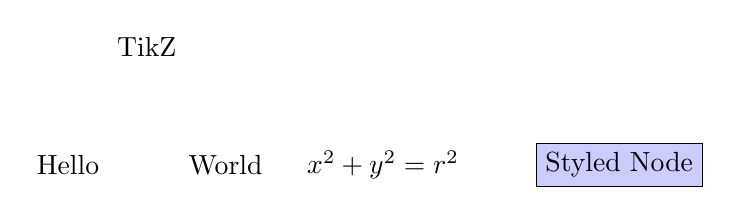
\begin{tikzpicture}[scale=1]

  % --- Simple text node ---
  \node at (0,0) {Hello};

  % --- Multiple nodes ---
  \node at (2,0) {World};
  \node at (1,1.5) {TikZ};

  % --- Node with math content ---
  \node at (4,0) {$x^2 + y^2 = r^2$};

  % --- Node with styling (box + fill) ---
  \node[draw, fill=blue!20] at (7,0) {Styled Node};

\end{tikzpicture}

\end{document}
